\chapter{Results \& Discussions}

All the published papers declared results for their experiment where the controllers were tested either for CPU or RAM utilization. They performed tests using the OFNet tool to create a virtual vast network and send a massive packets to the server and uses OFCProbe or OFCBench to monitor the CPU and RAM utilization via use of SMTP messages. However, instead of OFNet, multiple instances of CBench can also be used to send those packets.

In our experiment, we have used multiple instances of CBench and Mininet; and have also used Perf to read the system utilization information directly at the server.

After having our experiment as per the workflow depicted in Fig. \ref{workflowexperiment}, the collected raw data is clearly represented in graphical format. The system metrics that we collected and processed are as CPU Utilization, Clock Speed, Instructions per Second, Branch mispredictions and various level cache miss rates. These results are further discussed one by one.

/section{CPU Utilization}

Below are some snapshots of the experiment setup and commands used for the benchmark procedure.
Each controller operating system needs to be run in a virtual machine with dedicated RAM and processing power. A virtual box was used for this purpose.

The Floodlight controller was deployed by means of a ISO disk image in the virtual box on port 6633, while it's virtual network adapter was connected to the host machine so that the benchmark tool (Cbench) can simulate network switches and seamlessly perform the assessment.

\begin{figure}[!hbt]
        \centering
        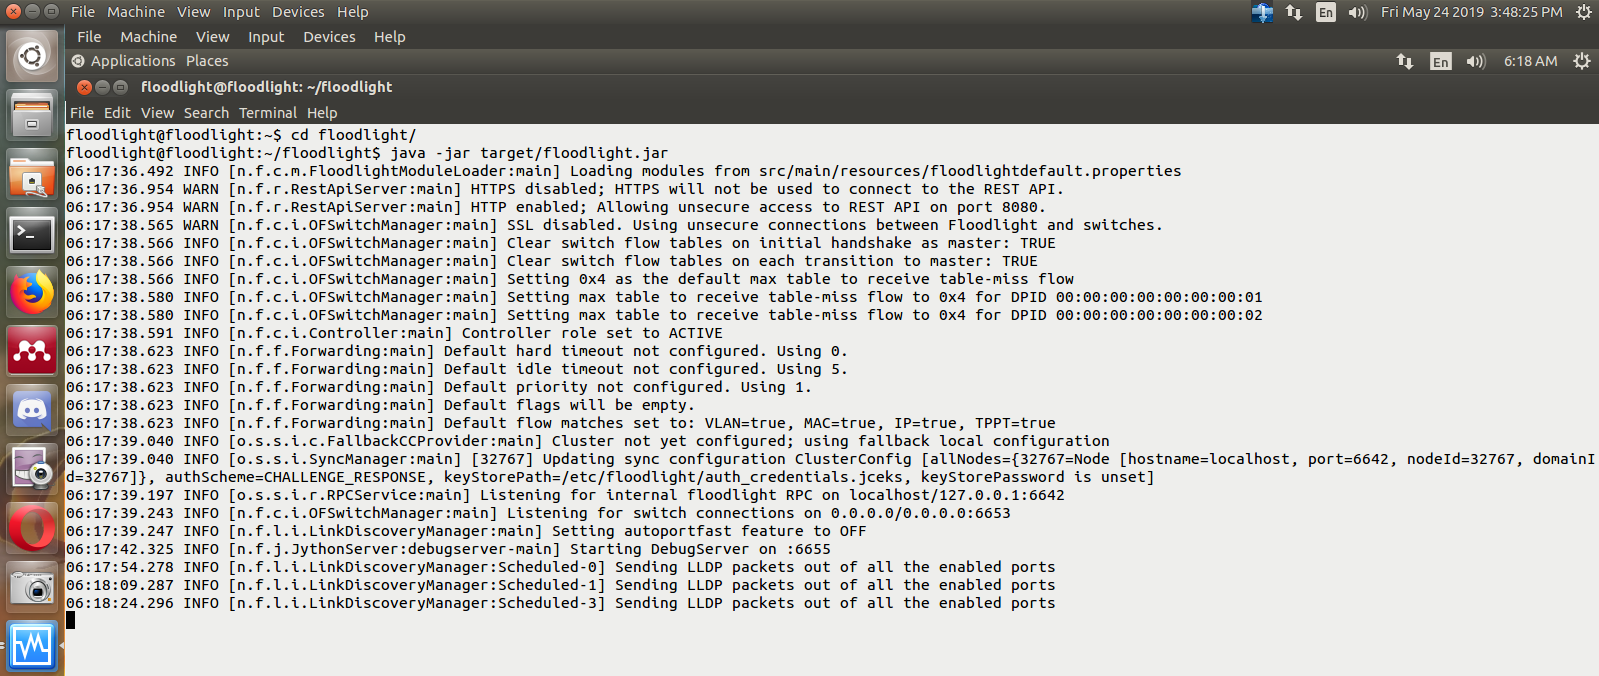
\includegraphics[width=\textwidth,keepaspectratio]{images/FL-Ctrl.png}
        \caption{Floodlight Controller Startup}
        \label{flsetup}
\end{figure}

\begin{figure}[!hbt]
        \centering
        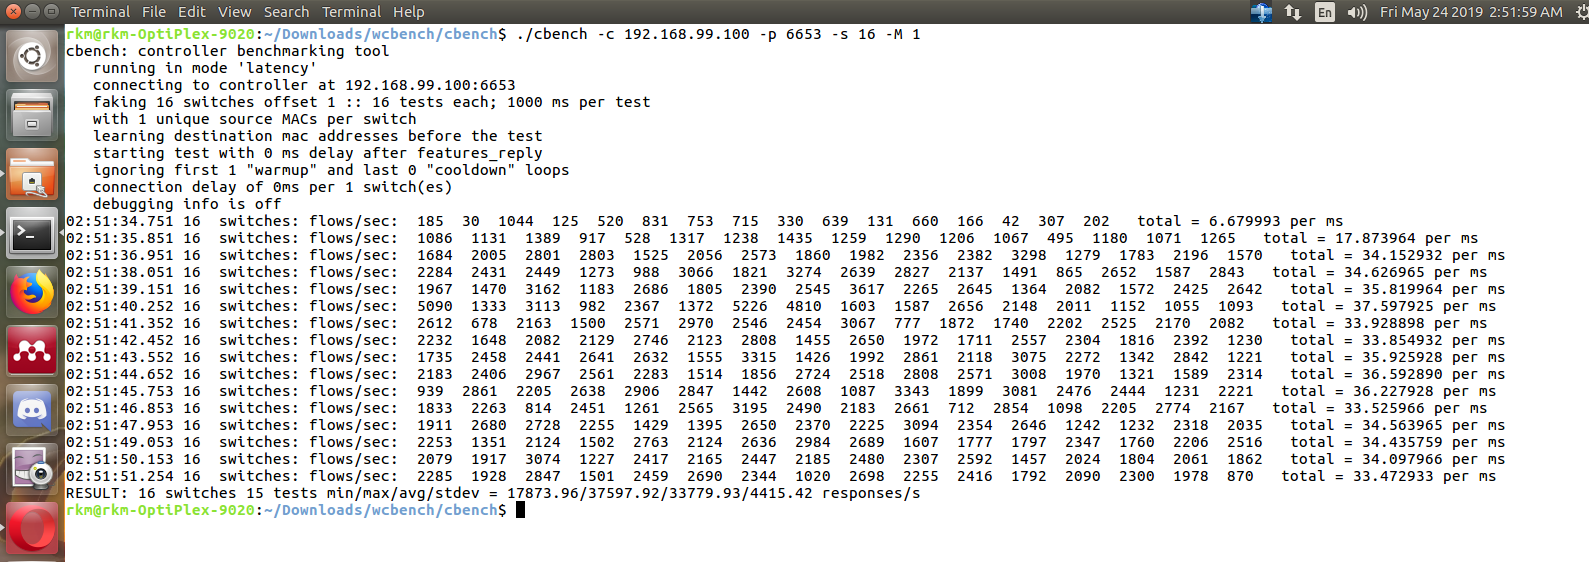
\includegraphics[width=\textwidth,height=0.5\textwidth]{images/FL-TP-16-to-1.png}
        \caption{Floodlight test scenario, Switch to Host ratio 16:1}
        \label{flrun}
\end{figure}

Secondly, the OpenVSwitch controller was run in the mininet emulator on port 6633. Mininet came with a handful of built in controllers including OpenVSwitch with OpenFlow protocol v3.0 .

\begin{figure}[!hbt]
        \centering
        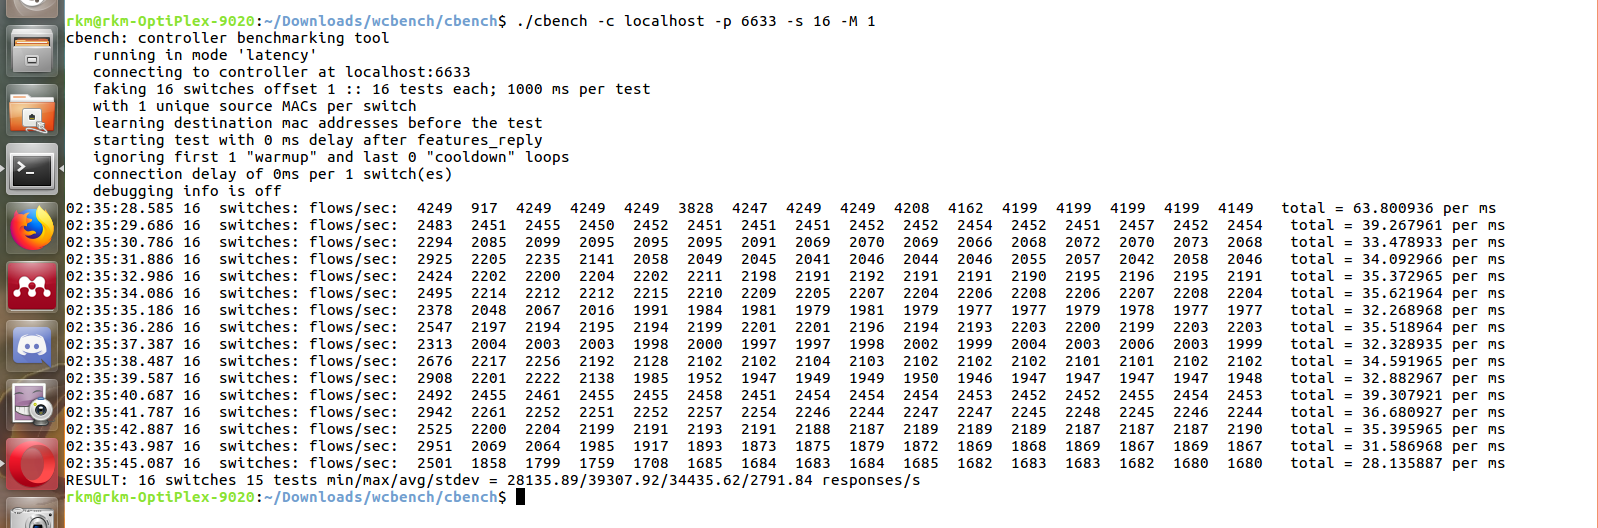
\includegraphics[width=\textwidth,height=0.5\textwidth]{images/OVS-TP-16-to-1.png}
        \caption{OpenVSwitch Test Case with the host to switch ratio 16:1}
        \label{ovsrun}
\end{figure} 

Lastly, the OpenDayLight controller operating system was deployed in a fedora virtual machine package called 'Vagrant'. Vagrant came with a preset configuration to deploy the controller and be able to benchmark within the virtual machine without affecting the performance of the controller by using a tool 'WCBench'. WCBench is a wrapped framework of CBench functions which provide results much easier.

\begin{figure}[!hbt]
        \centering
        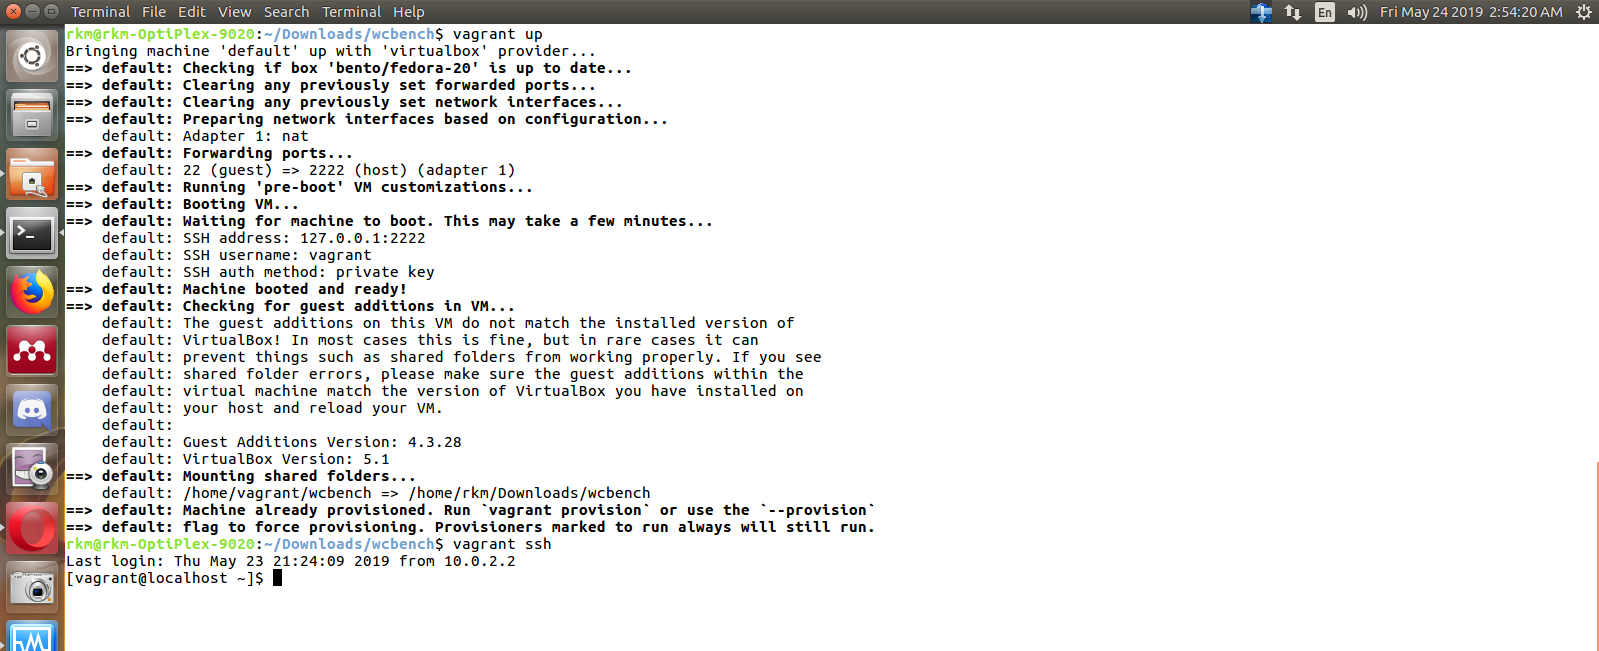
\includegraphics[width=\textwidth,height=0.5\textwidth]{images/vagrant-up-ssh.png}
        \caption{Open Day Light Setup in Vagrant VM}
        \label{vagup}
\end{figure}

\begin{figure}[!hbt]
        \centering
        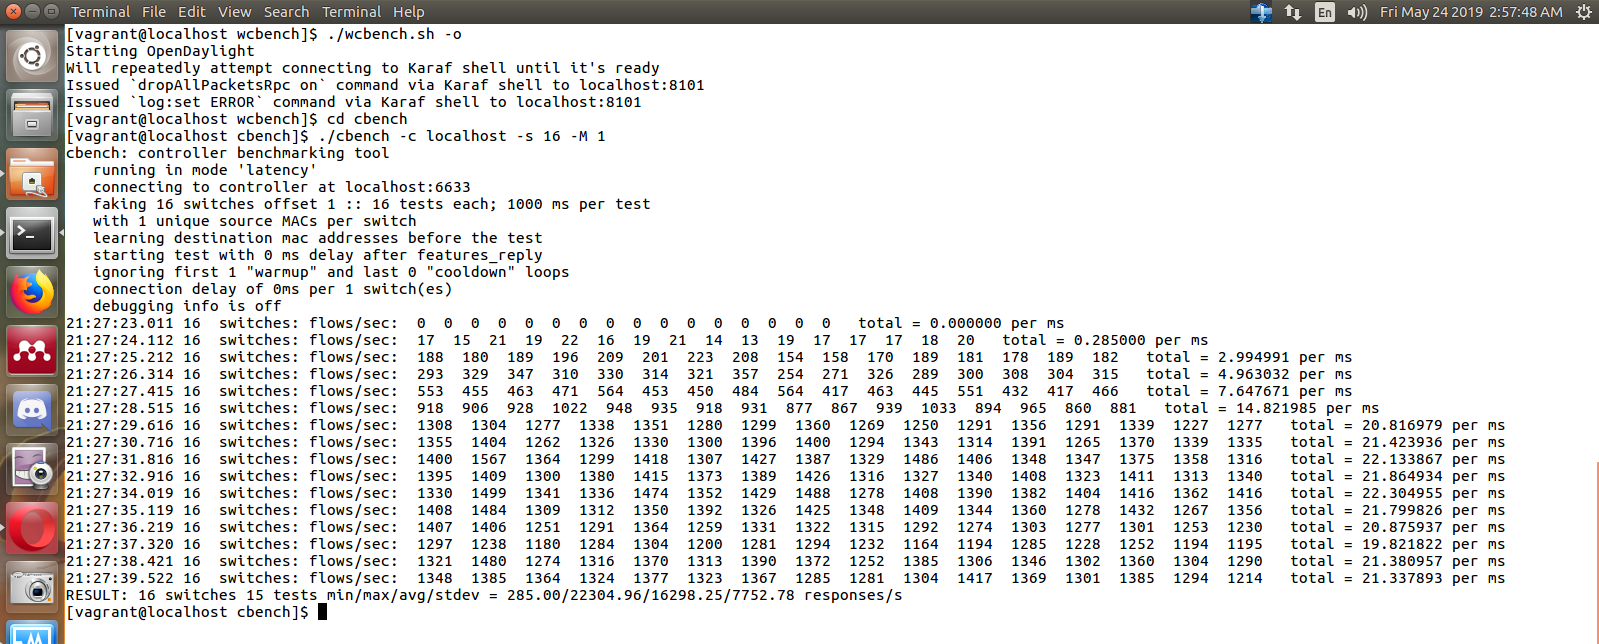
\includegraphics[width=\textwidth,keepaspectratio]{images/ODL-SSH-16-to-1.png}
        \caption{OpenDayLight test case in Vagrant VM}
        \label{vagrun}
\end{figure}
\vspace{5mm}
The data obtained from all the test cases for each controller were consolidated and plotted in a graph given below.The results below show us the performance of three controllers. OpenVSwitch (blue), Floodlight (red) and OpenDayLight (yellow). The two graphs together represent many network scenarios ranging from low-load \& less complex networks to high-load \& very complicated networks. 

The graph has a Y-axis showing response/sec from controller to switch with respect to X-axis values which are number of switches to number of host. The X-axis represents networks from left to right in order of complexity in both graphs. The graph representing results in throughput mode represents the raw performance of the controller when it is stressed with bulk requests. The graph representing results in latency mode depicts the delayed responses of controllers between requests when they are sent one by one.
The graph shows us a network topology based performance results by removing the factor of increasing traffic intensity from the equation as it maintains the total number of hosts in each test case.

\begin{figure}[!hbt]
        \centering
        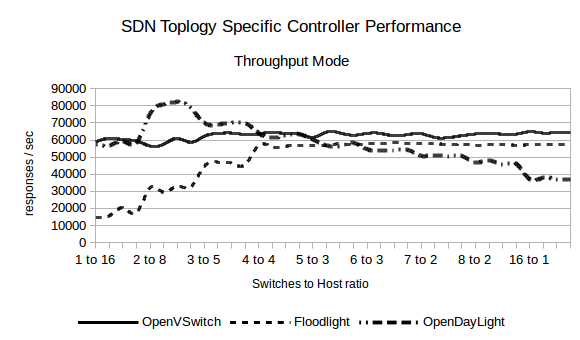
\includegraphics[width=0.85\textwidth,keepaspectratio]{ThroughputMode.png}
        \caption{SDN Throughput Mode Performance Results}
        \label{cnst_tpm}
\end{figure}

\begin{figure}[!hbt]
        \centering
        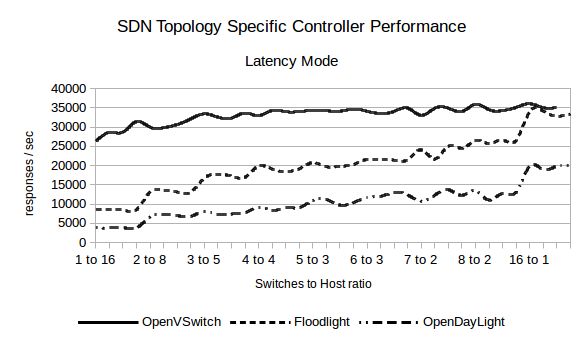
\includegraphics[width=0.85\textwidth,keepaspectratio]{LatencyMode.png}
        \caption{SDN Latency Mode Performance Results}
        \label{cnst_laten}
\end{figure}